\documentclass[A4paper, 11pt]{book}
\usepackage{atm_config}

\title{Appunti del corso di 
	\\ \Huge Fisica dell'Atmosfera}
\author{A cura di Lorenzo Uboldi}
\makeindex
\begin{document}
\frontmatter
\maketitle

	
% Colophon
\null % Bisogna inserire qualcosa prima di \vfill, altrimenti non funziona
\vfill % Riempie lo spazio verticale della pagina
\hspace*{-1.5em}\includegraphics[scale=.7]{figures/by-sa.eps}
\begin{flushleft}
	Quest'opera è stata rilasciata con licenza \emph{Creative Commons} Attribuzione - Condividi allo stesso modo 4.0 Internazionale. Per leggere una copia della licenza visita il sito web \url{https://creativecommons.org/licenses/by-sa/4.0/}.\\[1cm]
	Versione aggiornata al \today,\\
	Lorenzo Uboldi (\href{mailto:lorenzo.uboldi@studenti.unimi.it}{\ttfamily lorenzo.uboldi@studenti.unimi.it}), Milano.\\[0.2cm]
	L'ultima versione, aggiornata e rivista, è sempre disponibile a: \url{https://github.com/ulorentz/FisicaAtmosfera}
	
\end{flushleft}

\cleardoublepage

\tableofcontents
\mainmatter
\chapter{Pressione}
L'evidenza della pressione atmosferica può essere mostrata, ad esempio, con un barometro di Torricelli: capovolgendo un tubo con una sola apertura pieno di mercurio in una bacinella con lo stesso liquido, il livello del mercurio scende fino ad assestarsi ad una determinata altezza. La pressione atmosferica esercita una forza sul liquido nella bacinella che si oppone al peso che farebbe scendere il mercurio nel tubo. Precisamente, se $P_{B}$ è la pressione sulla bacinella e $P_{A}$ è quella esercitata dal mercurio nel tubo, $S$ è la sezione del tubo e $h_{\ch{Hg}}$ l'altezza della colonna di mercurio, all'equilibrio idrostatico si ha:
\begin{equation}
	P_{B}=P_{atm}=P_{A}=\frac{m_{\ch{Hg}}g}{S}=\frac{\rho_{\ch{Hg}} S h_{\ch{Hg}} g}{s}=\rho_{\ch{Hg}} h_{\ch{Hg}} g 
\end{equation}
il mercurio si assesta ad un'altezza di 76 cm, che corrispondono alla pressione media atmosferica di 1013 hPa.
\section{Origine della pressione atmosferica}
Supponiamo di avere un'atmosfera composta da un'unica particella di massa $m$ ad altezza $h$ rispetto alla superficie terrestre; inizialmente ferma, essa cade e subisce un urto elastico. La legge oraria è
\begin{equation}
	y(t)=h-\frac{1}{2}gt^2
\end{equation}
mentre la velocità finale all'impatto impatto della particella è
\begin{equation}
	v_f=\sqrt{2gh}.
\end{equation} 

Detto $\hat{j}$ il versore ortogonale uscente dalla superficie terrestre, la variazione di velocità è
\begin{align}
	\Delta \vec{v}=2\sqrt{2gh}\hat{j}
\end{align}
per cui, dato che il tempo che la particella impiega a cadere e tornare alla posizione iniziale è $t=2\sqrt{2h/g}$, la forza media che riceve è:
\begin{equation}
	\langle\vec{F}\rangle=\frac{m\Delta\vec{v}}{t}=\frac{2m\sqrt{2gh}\hat{j}}{2\sqrt{2h/g}}=mg\hat{j}.
\end{equation}

Per il terzo principio della dinamica, la forza media che riceve il pianeta è l'opposto, ovvero $\langle\vec{F}\rangle=-mg\hat{j}$. Nel caso di molte molecole, invece della massa della singola particella, si ha:
\begin{equation}
	\vec{F}=-M_{atm}g\hat{j}
\end{equation}
dove $M_{atm}\simeq 5.26 \cdot 10^{18}$kg.

L'origine della pressione atmosferica, dunque, è dovuta all'attrazione gravitazionale sulle molecole d'aria. 
\section{Equilibrio idrostatico in atmosfera}
Dal momento che l'atmosfera è estesa, essa interagisce con sè stessa: gli strati superiori comprimono quelli inferiori. La pressione, pertanto, varia lungo la coordinata zeta. 

Consideriamo una colonna di atmosfera come in figura (INSERIRE), se lo strato di aria compreso tra il punto A e B, la cui superficie di base è $S$, si trova in equilibrio dinamico, allora vale che $\sum\vec{F}=0$. Supponendo che la pressione sia costante lungo le coordinate $x$ e $y$, ovvero che $P=P(z)$, si ha la condizione\footnote{Nota che la pressione subita da un elemento di fluido è sempre diretta verso l'interno}
\begin{equation}\label{eq1}
	(\sum\vec{F})_z=P_A S - P_B S -mg =0.
\end{equation}

Considerata una variazione infinitesima lungo $z$, la pressione in B è 
\begin{equation}
	P_B=P_A+\frac{\partial P}{\partial z}dz
\end{equation}
e l'equazione \eqref{eq1} diviene
\begin{align}
	&P_A S - P_A S -\frac{\partial P}{\partial z}dzS -\rho S g dz=0\\
	&\Rightarrow -\frac{\partial P}{\partial z}-\rho g =0.
\end{align}
Se $P=P(z)$ (ovvero non dipende dalle componenti $x$ e $y$) si ha l'\emph{equazione di equilibrio idrostatico}:
\begin{equation}\label{idro}
	dP=-\rho g dz.
\end{equation}

In tre dimensioni, la forza dovuta alla pressione che subisce un elemento di atmosfera è\footnote{in fisica dell'atmosfera conviene ragionare in termini di unità di massa, in modo da eliminare la dipendenza da quest'ultima.}
\begin{equation}
	\frac{\vec{F}_P}{m}=-\frac{1}{\rho}\left(\frac{\partial P}{\partial x},\frac{\partial P}{\partial y}, \frac{\partial P}{\partial z}\right)
\end{equation}
ovvero
\begin{equation}
	\frac{\vec{F}_P}{m}=-\frac{1}{\rho}\nabla P.
\end{equation}

L'atmosfera organizza l'evoluzione della pressione ($\nabla P$) al fine di contrastare la forza gravitazionale, è da notare che $\frac{\partial P}{\partial z}$ è ordini di grandezza più grande delle altre componenti; inoltre, lungo la coordinata $z$, la pressione deve necessariamente decrescere affinché vi sia equilibrio. 

\section{Variazione della pressione lungo la coordinata $z$}
Dividendo ambo i lati dell'equazione dei gas perfetti per la massa, si ottiene:
\begin{equation}\label{gas}
	\frac{PV}{m}=\frac{n RT}{m} \rightarrow \frac{P}{\rho}=\frac{R}{M}T
\end{equation}
dove $M$ è la massa molare. Si noti che l'equazione dei gas perfetti è accurata quando si è lontani dai cambiamenti di stato, per le maggiori componenti dell'atmosfera (\ch{O_2} e \ch{NO_2}) questo è sicuramente vero. 

Inserendo la \eqref{gas} nell'equazione dell'equilibrio idrostatico \eqref{idro}, si ottiene:

\begin{equation}\label{dp}
	dP=-\frac{PM}{RT}g dz,
\end{equation}
dove $M$ è la massa molare. Considerati i maggiori componenti atmosferici, ovvero 75\% di azoto ($M_{N_2}=28$g/mol) e circa 25\% di ossigeno ($M_{O_2}=32$g/mol), si ottiene una media ponderata di $M=29$g/mol$=2.9\cdot10^{-2}$kg/mol.

Per ottenere l'andamento della pressione al variare della coordinata $z$, è necessario risolvere l'equazione differenziale \eqref{dp}. Il problema è che, in atmosfera, la temperatura è a sua volta dipendente della quota, ovvero $T=T(z)$, e, a priori, non è una funzione nota.\\


\subsection{Ipotesi di atmosfera isoterma}
L'andamento della temperatura in funzione della quota è, grossolanamente, rappresentato in figura (INSERIRE). Una tecnica per risolvere la \eqref{dp} è di considerare una temperatura media $\bar{T}$ dell'atmosfera, ad esempio di 250K, e di supporla, quindi, isoterma. 

Integrando la \eqref{dp}, si ottiene: 
\begin{align}
	\int_{P_0}^{P}\frac{dP'}{P'}&=-\int_{0}^{z}\frac{Mg}{R\bar{T}}dz'\\
	\ln P \Big|_{P_0}^P&=-\frac{Mg}{R\bar{T}}z\Big|_0^z\\
	P&=P_0\exp\left(-\frac{Mg}{R\bar{T}}z\right) \label{pz}.
\end{align}

Dalla \eqref{pz}, si intuisce che a temperature maggiori la pressione varia più lentamente all'aumentare della quota rispetto a temperature inferiori, e viceversa. Difatti, maggiore è la temperatura minore è il coefficiente che moltiplica $z$ nell'esponenziale.\\ %TODO inserire figura?

Un utilizzo della formula \eqref{pz} è per riportare le pressioni al livello del mare. Ogni stazione meteorologica è situata ad una specifica quota e per confrontare i valori di pressione rilevati in diverse coordinate geografiche è necessario confrontare dati alla stessa $z$. In altre parole per studiare $\frac{\partial P}{\partial x}$ e $\frac{\partial P}{\partial y}$ è necessario che $z$ sia costante.

Ad esempio, si supponga di effettuare una rilevazione a Linate (la cui altitudine è $z=104$m) di $P=1006.4$hPa ad una $T=10^\degree$C. Per calcolare la pressione al livello del mare:

\begin{equation*}
	P(-104\text{m})=1006.4\text{hPa}\cdot\exp\left(\frac{-29\cdot10^{-3}\text{kg/mol}\cdot 9.81\text{m/s}^2\cdot (-104\text{m})}{8.314\text{J/(mol K)} \cdot293.5 \text{K}}\right)=1019.1\text{hPa}
\end{equation*}
Da notare che la temperatura utilizzata è quella alla quota media tra l'altitudine della stazione e il livello del mare, e dal momento che nei primi strati di atmosfera il gradiente termico è di circa $0.65$K ogni 100m, si ha: $T_{media}=(283.15+0.65/2)\text{K}\sim 283.5$K.

Si deduce che, nello strato inferiore dell'atmosfera, il gradiente di pressione è di circa 12hPa ogni 100m, o anche 8 metri ogni hPa.\\

La \eqref{dp} può essere integrata per ricavare la dipendenza dalla quota dalla pressione, in situazioni come gli \emph{atmospheric soundings}\footnote{Sono dei palloni aerostatici pieni di elio che vengono lasciati liberi al fine di misurare i parametri atmosferici, ad esempio la pressione e temperatura.}, la variabile indipendente è proprio la pressione e non la coordinata $z$:
\begin{equation}
	\int_{z_1}^{z_2}dz=-\frac{RT}{Mg}\int_{P_1}^{P_2}\frac{dP}{P},
\end{equation}
ovvero
\begin{equation}
	z_2-z_1=-\frac{RT}{Mg}\ln \frac{P_2}{P_1}.
\end{equation}

Dalla \eqref{dp} si ottiene la dipendenza della densità atmosferica dalla variazione della pressione rispetto alla quota:
\begin{equation}
\rho=-\frac{1}{g}\frac{dP}{dz}.
\end{equation}
Utilizzando la \eqref{pz} si ha
\begin{equation}
\rho=-\frac{1}{g}P_0\left(-\frac{Mg}{RT}\right)e^{-\frac{Mg}{RT}z}
\end{equation}
ovvero, ricavando dall'equazione dei gas perfetti $\rho_0=\frac{P_0 M}{RT}$:
\begin{equation}\label{roz}
\rho=\rho_0 e^{-\frac{Mg}{RT}z}.
\end{equation}

La grandezza $z_0=\frac{RT}{Mg}$ viene chiamata \emph{altezza di scala} (quota necessaria affinché la pressione e la densità si abbattano di un fattore 1/e), le equazioni \eqref{pz} e \eqref{roz} possono essere riscritte come:
\begin{align}
P&=P_0e^{-\frac{z}{z_0}}\\
\rho&=\rho_0e^{-\frac{z}{z_0}}.
\end{align}

\subsection{Ipotesi di dipendenza lineare della temperatura}
Nella troposfera la dipendenza della temperatura con la quota è sufficientemente lineare (FIGURA) da poter considerare la seguente relazione:
\begin{equation}\label{tz}
	T(z)=T_0-\gamma z
\end{equation}
dove $\gamma=6.5$K/km è detto \emph{gradiente troposferico medio}.

Utilizzando la \eqref{tz} nella \eqref{dp} ed integrando, si ha:
\begin{align}
	\int_{P_0}^{P}\frac{dP'}{P'}&=-\int_{0}^{z}\frac{Mg}{R(T_0-\gamma z')}dz'\\
	\ln P'\Big|_{P_0}^P&=-\frac{Mg}{R}\left( -\frac{1}{\gamma}\right)\int_{0}^{z}\frac{dz'}{z'-T_0/\gamma}=\frac{Mg}{R\gamma}\ln\left|z'-\frac{T_0}{\gamma}\right|^z_0\\
	\ln\frac{P}{P_0}&=\frac{Mg}{R\gamma}\ln\left(\frac{\frac{T_0}{\gamma}-z}{\frac{T_0}{\gamma}}\right)=\frac{Mg}{R\gamma}\ln\left(\frac{T(z)}{T_0}\right)\\
	P(z)&=P_0\left(\frac{T(z)}{T_0}\right)^{\frac{Mg}{R\gamma}}\\
\text{invertendo si ottiene:}\nonumber\\
	z(P)&=\frac{T_0}{\gamma}\left(1-\left(\frac{P}{P_0}\right)^{\frac{R\gamma}{Mg}}\right).\label{zp}
\end{align}\\

Anche in questo caso è possibile esplicitare la dipendenza della densità dalla quota, utilizzando la \eqref{zp} si ricava:
\begin{align}
	\rho&=-\frac{1}{g}P_0\left(\frac{Mg}{R\gamma}\right)\left(\frac{T(z)}{T_0}\right)^{\frac{Mg}{R\gamma}-1}\left(\frac{\gamma}{T_0}\right)\\
	\rho&=\rho_0\left(\frac{T(z)}{T_0}\right)^{\frac{Mg}{R\gamma}-1}\label{rho}
\end{align}
dove si è utilizzato $\rho_0=\frac{P_0M}{RT}$.

Si noti che nell'atmosfera reale il gradiente termico non è costante, l'esponente della \eqref{rho} pertanto può annullarsi: in questa situazione la densità atmosferica è costante al variare della quota. L'esponente, però, non può mai essere negativo: fisicamente la statica dei fluidi impedisce una $\frac{\partial \rho}{\partial z} >0$ (l'atmosfera non sarebbe in equilibrio). Nella condizione limite in cui l'esponente si annulla si ha che $\gamma =\frac{Mg}{R}=0.034$K/m$=3.4$K$/100$m. Questo è il limite massimo che il gradiente termico può raggiungere, e proprio perché si perde la stabilità statica è detto \emph{gradiente autoconvettivo}. 

\subsubsection{Confronto tra le due ipotesi}
È utile confrontare i risultati ottenuti con l'ipotesi di atmosfera isoterma e di gradiente troposferico medio. 

Ipotizziamo di avere uno strato con $T_0=300$K,$P_0=1000$hPa, $P_{top}=200$hPa e $\bar{T}=260$K (temperatura media, necessaria per l'ipotesi di isotermia). Ci si chiede a che quota è il top dello strato. 
\begin{table}[h]
	\centering
	\begin{tabular}{c|c}
		Isoterma & Gradiente medio \\
		$z_{top}=-\frac{R\bar{T}}{Mg}\ln\frac{P_{top}}{P_0}$ & $z_{top}=\frac{T_0}{\gamma}\left(1-\left(\frac{P}{P_0}\right)^{\frac{R\gamma}{Mg}}\right)$\\
		= 12229 m & = 12157 m
	\end{tabular}
\end{table}

La situazione sopra esposta è rappresentata in figura \ref{fig:iso_vs_grad} da cui si deduce che le due ipotesi, in troposfera, sono in buon accordo. 

\begin{figure}[h]     				\centering                                                                  
   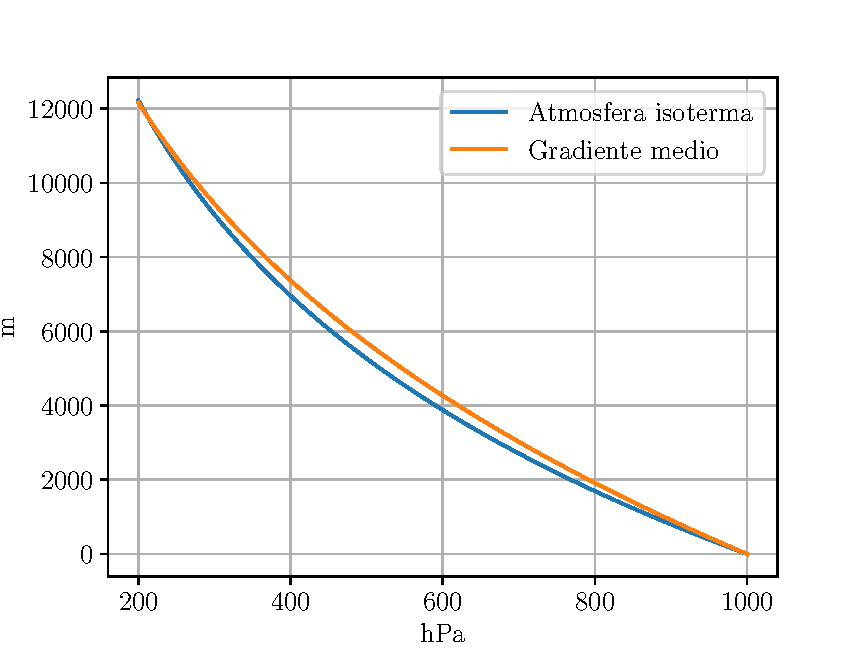
\includegraphics[width=.65\textwidth]{figures/iso_vs_grad.pdf} 
	\caption{Confronto tra atmosfera isoterma e ipotesi di gradiente troposferico medio}          
   \label{fig:iso_vs_grad}
\end{figure}         



\chapter{Dinamica dell'Atmosfera}
L'equazione che regola la relazione tra forze e pressione, e quindi la dinamica dell'atmosfera, è
\begin{equation}\label{fpress}
\frac{\vec{F}_p}{m}=-\frac{1}{\rho}\nabla P.
\end{equation}

Nel capitolo precedente è stato analizzato l'andamento della componente verticale del gradiente di pressione, il cui scopo è mantenere in equilibrio l'atmosfera; è lecito chiedersi, invece, quale sia la causa delle componenti orizzontali.

Generalmente, diverse temperature causano variazioni di pressione, ovvero
\begin{equation*}
\nabla_{orizz} T \Rightarrow \nabla_{orizz} P
\end{equation*}
questo fenomeno è detto \emph{baroclinicità}. Questo si configura in gradienti di pressione originati da gradienti di temperatura. Gli ultimi sono dovuti, ad esempio, a diverse composizioni del terreno dotati di capacità termiche differenti; a diverse esposizioni solari; a bacini idrici, ecc\ldots  È da notare che su grandi scale si ha generalmente $\frac{\partial T}{\partial y} > \frac{\partial T}{\partial x}$.\\

Per comprendere l'andamento del gradiente di pressione orizzontale su grandi scale, può essere utile studiare le carte delle isobare. Da queste, infatti, si osservano alcune strutture tipiche, ovvero i cicloni, gli anticicloni, le saccature e i cunei. (INSERIRE FIGURE).

Il ciclone è una struttura circolare che si forma attorno ad un centro di bassa pressione: dalle carte si osserva che i venti seguono le isobare circolando in senso antiorario, con una leggera tendenza alla convergenza verso il centro. 

L'anticiclone si sviluppa in zone di alta pressione, i venti circolano in senso orario, seguendo le isobare, con una leggera tendenza a divergere dal centro.
\section{Forze non inerziali: origine delle strutture circolari}
Si ipotizzi che vi sia solo il gradiente di pressione, in tal caso sul piano orizzontale vi è una forza perpendicolare alle isobare e diretta verso la bassa pressione la cui formula è
\begin{equation}
\frac{(\vec{F}_P)_{horiz}}{m}=-\frac{1}{\rho}\nabla P.
\end{equation}

A scopo di esempio, si supponga la presenza di un $\delta P = 8$ hPa per un $\delta x=400$km, allora si ha: $\frac{\partial P}{\partial x}=2\cdot10^{-3}$Pa/m. Inserendo nella formula precedente, si ottiene in modulo $\left(\frac{\vec{F}_P}{m}\right)_x = -\frac{1}{\rho}\frac{\partial P}{\partial x}\sim 2\cdot 10^{-3}$m/s$^2$. Se non vi fossero altre forze, quest'ultima non sarebbe contrastata e, spostando masse d'aria, andrebbe ad appianare i gradienti di pressione causati da gradienti di temperatura, uniformando l'atmosfera. 

Nel precedente ragionamento si è trascurato il fatto che la Terra non è un sistema di riferimento inerziale e, pertanto, sono presenti ulteriori forze.

(INSERIRE FIGURA TERRA E SISTEMA RIFERIMENTO)
Un punto nel sistema di riferimento terrestre (non inerziale) detto $O'$, rispetto ad un sistema di riferimento inerziale è:
\begin{align}
	\vec{R}&=\vec{OP}(t)=\vec{O'P}(t)+\vec{OO'}\\
	\vec{a}_{assoluta}&=\vec{a}_{rel}+2\vec{\Omega}\times\vec{v}_r+\vec{\Omega}\times(\vec{\Omega}\times\vec{R})
\end{align}
dove $\vec{a}_{rel}$ è quella del sistema non inerziale. Segue che
\begin{align}
	\frac{\sum \vec{F}}{m}=\vec{a}_{as}=\vec{a}_{rel}+2\vec{\Omega}\times\vec{v}_{rel}+\vec{\Omega}\times(\vec{\Omega}\times\vec{R})\\
	\vec{a}_{rel}=\frac{\sum \vec{F}}{m}+\frac{-2m\vec{\Omega}\times\vec{v}_{rel}-m\vec{\Omega}\times(\vec{\Omega}\times\vec{R})}{m}\label{arel}.
\end{align}
Pertanto, è possibile considerare $\vec{a}_{rel}$, ovvero quella del sistema non inerziale solidale alla Terra, a patto di aggiungere il secondo termine alle forze:
\begin{equation}
	\vec{a}=\frac{\sum\vec{F}_{rel}+\sum\vec{F}_{app}}{m}.
\end{equation}
\subsection{Forza centrifuga}
Il termine $\vec{\Omega}\times(\vec{\Omega}\times\vec{R})$ rappresenta la forza centrifuga. Quest'ultima vale in modulo  $|F_c|=\Omega^2 R\sin(\frac{\pi}{2}-\theta)$ ed è diretta ortogonalmente all'asse di rotazione terrestre, in verso uscente.

L'espressione della forza centrifuga, proiettata sugli assi, è
\begin{equation}\label{scomp_fc}
	-\vec{\Omega}\times(\vec{\Omega}\times\vec{R})=-\vec{\Omega}^2\vec{R}\sin\theta\cos\theta\hat{u}_\theta+\cos^2\theta\hat{u}_z.
\end{equation}
Si noti che il segno negativo a sinistra dell'uguale è coerente con la \eqref{arel}.

Dalla \eqref{scomp_fc} si evince che il secondo termine, massimo all'equatore, ha l'effetto di diminuire la forza gravitazionale; è da tener presente che l'ordine di grandezza è di $10^{-3}$ m/s$^2$, mentre le forze di pressione verticale sono dell'ordine di 10 m/s$^2$: pertanto, è del tutto trascurabile.

Sulla direzione y ($\hat{u}_\theta$ è diretto lungo tale asse), invece, non sono presenti forze così intense e l'effetto di $F_c$ è di spostare le masse verso l'equatore (il primo termine nella \eqref{scomp_fc}). La forza centrifuga esiste da miliardi di anni e la sua continua azione è risultata in una progressiva modificazione della forma del pianeta: la superficie terrestre si è allineata ad una  equipotenziale per la forza gravitazionale e centrifuga. In questo modo è stata contrastata la tendenza a spostare le masse verso l'equatore (DETTA BENE? CORRETTO?).

\subsection{Coriolis}
La forza di Coriolis è\footnote{Espressa con i segni coerenti con la \eqref{arel}} data da
\begin{align}
	-2\vec{\Omega}\times\vec{v}&=-2[(\vec{\Omega}_{\parallel}+\vec{\Omega}_\perp)\times(\vec{v}_\parallel+\vec{v}_\perp)]=\\
	&=-2[(\vec{\Omega}_\parallel\times\vec{v}_\parallel)+(\vec{\Omega}_\perp\times\vec{\Omega}_\parallel)+(\vec{\Omega}_\parallel\times\vec{\Omega}_\perp)+(\vec{\Omega}_\perp\times\vec{\Omega}_\perp)]
\end{align}
dove il primo e il quarto termine sono nulli per le proprietà del prodotto vettoriale. Inoltre, essendo $||\vec{v}||\approx||\vec{v}_\parallel||$ (ovvero $||\vec{v}_\parallel||>>||\vec{v}_\perp||$), si ha:
\begin{equation}\label{coriolis}
	\frac{(\vec{F_{cor}})_{horiz}}{m}\approx-2\vec{\Omega}_\perp\times\vec{v}_\parallel.
\end{equation}

Il modulo della \eqref{coriolis} è $2\Omega\sin\theta$; la direzione  è perpendicolare a $\vec{v}_\parallel$ e nel piano tangente alla Terra; il verso è a destra del vettore velocità. È da notare che il modulo è dello stesso ordine di grandezza di quello della forza di pressione: la differenza tra le due, invece, funge da forza centripeta.

\section{Forze di pressione, cambio di variabili}
Nell'equazione per le forze di pressione \eqref{fpress}, la variabile dipendente risulta la pressione, mentre quelle indipendenti sono le coordinate spaziali. Restringendosi alle componenti orizzontali\footnote{Si è visto come la componente verticale è organizzata in modo da compensare la forza gravitazionale: per lo studio della dinamica dell'atmosfera, è di particolare interesse la proiezione orizzontale.}, infatti, si ha:
\begin{equation}\label{forizz}
	\frac{(\vec{F}_P)_{horiz}}{m}=-\frac{1}{\rho}\left(\frac{\partial P}{\partial x},\frac{\partial P}{\partial y}\right).
\end{equation}

Sperimentalmente, nei rilevamenti delle termosonde, la situazione è invertita: la variabile indipendente dei sondaggi è la pressione da cui viene ricavata la quota. È necessario effettuare un cambio di variabili in modo da poter calcolare le forze di pressione orizzontali dai dati dei termosondaggi.

Denotiamo la nuova variabile come ``$s$''. Si consideri una situazione come in figura (FARE), ove il punto A e B sono ad $x$ diverse e $z$ uguale, mentre il punto C si trova alla stessa $x$ di B ma a quota superiore. Allora, valutando le derivate con la nuova variabile $s$ mantenuta costante, si ha:
\begin{align}
	\left(\frac{\partial P}{\partial x}\right)_s&=\lim_{c\to a}\frac{\partial P}{\partial x}=\lim_{c\to a}\frac{P_c-P_a}{x_c-x_a}=\lim_{c\to a}\frac{P_c-P_b}{x_c-x_a}+\frac{P_b-P_a}{x_c-x_a}=\\
		&=\lim_{c\to a}\frac{(P_c-P_b)(z_c-z_b)}{(z_c-z_b)(x_c-x_a)}+\frac{P_b-P_a}{x_c-x_a}=\left(\frac{\partial P}{\partial x}\right)_x \left(\frac{\partial z}{\partial x}\right)_s+\left(\frac{\partial P}{\partial x}\right)_z,
\end{align}
dove si è tenuto conto che $z_b=z_a$. Inserendo $s=P=cost$ e utilizzando l'equazione dell'equilibrio idrostatico \eqref{idro} per la derivata rispetto a $z$, si ottiene:
\begin{equation}
	0=-\rho g\left(\frac{\partial x}{\partial x}\right)_P+\left(\frac{\partial P}{\partial x}\right)_z \Rightarrow \left(\frac{\partial P}{\partial x}\right)_z=\rho g \left(\frac{\partial z}{\partial x}\right)_P
\end{equation}

Dopo aver ripetuto il ragionamento per la coordinata $y$, è possibile esprimere l'equazione \eqref{forizz} nelle nuove coordinate $(x, y, P)$:
\begin{equation}\label{newcoord}
	\left(\frac{\vec{F}_P}{m}\right)_{horiz}=-g\left(\frac{\partial z}{\partial x}, \frac{\partial z}{\partial y}\right)_{P=cost}
\end{equation}

\section{Gradienti di temperatura al suolo}
Si ipotizzi una situazione come quella descritta in figura (FARE): due zone limitrofe a quota zero si trovano a temperature diverse. La pressione al suolo è uguale ma, come si evince dall'equazione \eqref{pz}, l'andamento in quota diverge a causa della diversa temperatura.

Ad esempio, si consideri un'estesa area geografica con pressione al suolo costante, isoterme parallele all'asse $x$ e un importante gradiente di temperatura lungo la $y$: 
\begin{equation}
	\frac{\partial T}{\partial y}=a.
\end{equation}
L'andamento della temperatura dipende, dunque, dalle coordinate $y$ e $z$:
\begin{equation}
	T(y,z)=T_0+ay-\gamma z
\end{equation}
con $\gamma=6.5\degree$C/km. Nell'ipotesi che la temperatura si riduca linearmente con $z$, è possibile ricavare l'andamento della pressione; nonché invertire la relazione per esplicitare $z=z(x,y,P)$ in modo da calcolare le forze di pressione con la \eqref{newcoord}:
\begin{align}
&\frac{P}{P_0}=\left(\frac{T_0+ay-\gamma z}{T_0+ay}\right)^{\frac{gM}{R\gamma}}\\
&\left(\frac{P}{P_0}\right)^{\frac{R\gamma}{gM}}=1-\frac{\gamma z}{T_0+ay}\\
&z=\frac{T_0+ay}{\gamma}\left[1-\left(\frac{P}{P_0}\right)^{\frac{R\gamma}{Mg}}\right].
\end{align}
La variazione di $z$ rispetto alle due coordinate orizzontali è
\begin{equation}
	\frac{\partial z}{\partial x}=0 \qquad \frac{\partial z}{\partial y}=\frac{a}{\gamma}\left[1-\left(\frac{P}{P_0}\right)^{\frac{R\gamma}{Mg}}\right]
\end{equation}
ovvero, utilizzando la \eqref{newcoord}, la forza di pressione diretta lungo l'asse $y$ è:
\begin{equation}
	(\vec{F}_P)_y=-\frac{ag}{\gamma}\left[1-\left(\frac{P}{P_0}\right)^{\frac{R\gamma}{Mg}}\right].
\end{equation}

Ad un gradiente di temperatura al suolo, l'atmosfera risponde con un gradiente di pressione che cresce all'aumentare della quota. Quest'ultimo causa intese forze di pressione che, per essere bilanciate dalla forza di Coriolis, sviluppano venti estremamente intensi. 

Ad esempio, si consideri una pressione al suolo $P_0=1000$ hPa e un gradiente di temperatura di
\begin{equation}
\frac{\partial T}{\partial y}=-\frac{10\degree\text{C}}{500\text{km}},
\end{equation}
si ricavano i seguenti valori:
\begin{table}[h]
	\centering
	\begin{tabular}{c|c|c}
		$P$(hPa) & $(\vec{F}_P)_y$ (m/s$^2$) & $v$ (m/s)  \\ \hline
		1000 & 0 & 0 \\ \hline
		850  & $0.9 \cdot 10^{-3}$ & 9 \\ \hline
		700  & $2 \cdot 10^{-3}$ & 20 \\ \hline
		500  & $4\cdot 10^{-3}$ &40 \\ \hline
		200  & $8\cdot 10^{-3}$ & 80 
	
	\end{tabular}
\end{table}

\section{Vorticità}
Dato un campo vettoriale $\vec{v}(x,y,z)=(u, v, w)$, si definisce \emph{vorticità} il rotore del campo:
\begin{equation}
	\nabla \times \vec{v}=\hat{u}_\lambda\left(\frac{\partial w}{\partial y}- \frac{\partial v}{\partial z}\right) 
	+\hat{u}_\theta\left(-\frac{\partial w}{\partial x}+\frac{\partial u}{\partial z}\right)
	+\hat{u}_z\left(\frac{\partial v}{\partial x}-\frac{\partial u}{\partial y}\right).
\end{equation}

Ognuno dei termini a destra dell'uguale indica quanto rapidamente il campo ruota in senso antiorario attorno ai versori $\hat{u}$.

Per l'atmosfera, è difficile ruotare nei piani $(x,z)$ e $(y,z)$ in quanto, in molte situazioni, il gradiente termico verticale ne impedisce lo spostamento di grandi masse d'aria. Pertanto, i termini $\hat{u}_\lambda$ e $\hat{u}_\theta$ del gradiente sono spesso poco importanti e trascurabili, mentre domina $\mathcal{Z}:=(\nabla\times\vec{v})_z$. Approssimando una colonna d'aria ad un corpo rigido che ruota attorno all'asse $z$, si ha:
\begin{equation}
	\mathcal{Z}=\frac{Rw-(-Rw)}{2R}-\frac{(-Rw)-Rw}{2R}=2w.
\end{equation}
Se la colonna, idealizzata come un cilindro, è costretta a cambiare altezza (per esempio incontrando una catena montuosa da scavalcare), dal momento che il momento angolare si deve conservare, segue che
\begin{equation}
	L_z=Iw=\frac{1}{2}mR^2_1w_1=\frac{1}{2}mR^2_2w_2,
\end{equation}
e dividendo per il volume di entrambi i cilindri:
\begin{equation}
	\frac{w_1}{h_1}=\frac{w_2}{h_2}.
\end{equation}
Pertanto, una circolazione ciclonica può essere indotta dal fatto che la massa d'aria si allunga verticalmente. 

Inoltre, è necessario tenere in considerazione che la Terra è un sistema di riferimento non inerziale: oltre alla vorticità della massa d'aria bisogna tenere conto della rotazione terrestre nelle quantità conservate. Detta $\mathcal{F}_0=2\Omega\sin\theta$ la vorticità della Terra, la quantità conservata è:
\begin{equation}
	\frac{\mathcal{Z}+\mathcal{F}_0}{h}=\text{const}.
\end{equation}

La vorticità della Terra è nulla all'equatore e massima ai poli: può apparire che masse d'aria si mettano in rotazione da sole, ma il fenomeno è dovuto al cambiamento di $h$ o di $\mathcal{F}_0$.

Ad esempio, si supponga $h$ costante e si ipotizzi che una massa d'aria sia costretta a muoversi verso sud: $\mathcal{F}_0$ diminuisce e, per conservare la vorticità totale, $\mathcal{Z}$ aumenta e la massa d'aria si mette in rotazione rispetto alla terra con una circolazione ciclonica. L'esatto opposto avviene se è costretta a muoversi a nord. Tale fenomeno è osservabile nel flusso zonale: questo è un flusso da ovest ad est che avviene lungo i paralleli. In esso si intuiscono oscillazioni attorno ai paralleli dovute alla conservazione della vorticità (INSERIRE FIGURA).
\chapter{Climatologia}
\end{document}